%%%%%%%%%%%%%%%%%%%%%%%%%%%%%%%%%%%%%%%%%
% Beamer Presentation
% LaTeX Template
% Version 1.0 (10/11/12)
%
% This template has been downloaded from:
% http://www.LaTeXTemplates.com
%
% License:
% CC BY-NC-SA 3.0 (http://creativecommons.org/licenses/by-nc-sa/3.0/)
%
%%%%%%%%%%%%%%%%%%%%%%%%%%%%%%%%%%%%%%%%%

%----------------------------------------------------------------------------------------
%	PACKAGES AND THEMES
%----------------------------------------------------------------------------------------

\documentclass{beamer}
\mode<presentation> {

% The Beamer class comes with a number of default slide themes
% which change the colors and layouts of slides. Below this is a list
% of all the themes, uncomment each in turn to see what they look like.

%\usetheme{default}
%\usetheme{AnnArbor}
%\usetheme{Antibes}
%\usetheme{Bergen}
%\usetheme{Berkeley}����JFIF����C
%\usetheme{Berlin}
%\usetheme{Boadilla}
%\usetheme{CambridgeUS}
%\usetheme{Copenhagen}
%\usetheme{Darmstadt}
%\usetheme{Dresden}
%\usetheme{Frankfurt}
%\usetheme{Goettingen}
%\usetheme{Hannover}
%\usetheme{Ilmenau}
%\usetheme{JuanLesPins}
%\usetheme{Luebeck}
%\usetheme{Madrid}
%\usetheme{Malmoe}
%\usetheme{Marburg}
%\usetheme{Montpellier}
\usetheme{PaloAlto}
%\usetheme{Pittsburgh}
%\usetheme{Rochester}
%\usetheme{Singapore}
%\usetheme{Szeged}
%\usetheme{Warsaw}

% As well as themes, the Beamer class has a number of color themes
% for any slide theme. Uncomment each of these in turn to see how it
% changes the colors of your current slide theme.

%\usecolortheme{albatross}
%\usecolortheme{beaver}
%\usecolortheme{beetle}
%\usecolortheme{crane}
%\usecolortheme{dolphin}
%\usecolortheme{dove}
%\usecolortheme{fly}
%\usecolortheme{lily}
%\usecolortheme{orchid}
%\usecolortheme{rose}
%\usecolortheme{seagull}
%\usecolortheme{seahorse}
\usecolortheme{whale}
%\usecolortheme{wolverine}

%\setbeamertemplate{footline} % To remove the footer line in all slides uncomment this line
\setbeamertemplate{footline}[page number] % To replace the footer line in all slides with a simple slide count uncomment this line

%\setbeamertemplate{navigation symbols}{} % To remove the navigation symbols from the bottom of all slides uncomment this line
}

\usepackage{graphicx} % Allows including images
\usepackage{booktabs} % Allows the use of \toprule, \midrule and \bottomrule in tables
\usepackage{amsmath}
\usepackage{subfig}
\usepackage{caption}
\usepackage{mathabx}
\usepackage{wrapfig}
\usepackage{tikz}
\usepackage{animate}
\usepackage{adjustbox}
\usetikzlibrary{shapes.geometric, arrows}
%\usepackage{subcaption}
%----------------------------------------------------------------------------------------
%	TITLE PAGE
%----------------------------------------------------------------------------------------
\title[]{``Club of looking for jobs'' and duration of unemployment of females} % The short title appears at the bottom of every slide, the full title is only on the title page

\author{Alexander Dudoladov, Adel Khusnulgatin, Alexander Petrov} % Your name
\institute[New Economic School] % Your institution as it will appear on the bottom of every slide, may be shorthand to save space
{
New Economic School \\ % Your institution for the title page
\medskip
%\textit{john@smith.com} % Your email address
}
\date{\today} % Date, can be changed to a custom date

\begin{document}

\begin{frame}
\titlepage % Print the title page as the first slide
\end{frame}

%--------------------------------------------------------------------------------
\section{Introduction}

%GitHub check

\begin{frame}{Hypotheses}
\begin{block}{What is the impact of participation in "Club of looking for jobs" program on duration of unemployment of females?}
\begin{itemize}
       \item Program helps individuals to find a job
       \item Negative impact on observed duration of unemployment in the given sample
\end{itemize}
\end{block}
\end{frame}

\begin{frame}{Club of looking for jobs}
\begin{block}{Target audience}
\begin{itemize}
       \item Currently unemployed
       \item Lost their motivation
\end{itemize}
\end{block}

\begin{block}{Main goal: help people to find appropriate jobs}
\begin{itemize}
       \item Business speech
       \item Make people believe in competence
       \item Teach how to set and achieve a goal
       \item Motivate to find a job
\end{itemize}
\end{block}

\end{frame}

\begin{frame}{Other conjectures}
\begin{block}{Self selection?}
\begin{itemize}
    \item Those who join the club are different from others
    \item This decision is endogenous
\end{itemize}
\end{block}

\begin{block}{Biased estimates?}
\begin{itemize}
    \item Clubs might be helpful but estimates are biased
    \item Control group should be marginally close to the club
\end{itemize}
\end{block}
\end{frame}

\section{Data}

\begin{frame}{Data}
\begin{block}{Voronezh dataset, single record observations}
\begin{itemize}
    \item Covered period: 1994 - 2000
        \begin{itemize}
            \item  240 726 observations in total
            \item  145 796 females
            \item  2 290 participants of the club
            \item  1 933 females in the club
        \end{itemize}
\end{itemize}
\end{block}
\end{frame}







%---------------------------------------------------------------------------
\begin{frame}{Summary statistics}
\centering
\resizebox{0.9\linewidth}{!}{
{
\def\sym#1{\ifmmode^{#1}\else\(^{#1}\)\fi}
\begin{tabular}{l*{3}{c}}
\toprule
 & Not in the club & In the club \\
\midrule
Age             &    34.01 & 33.52\\
Number of dependants &    0.54 & 0.61\\
\bottomrule
\end{tabular}
}

}
\end{frame}




\begin{frame}{Distribution by status}
    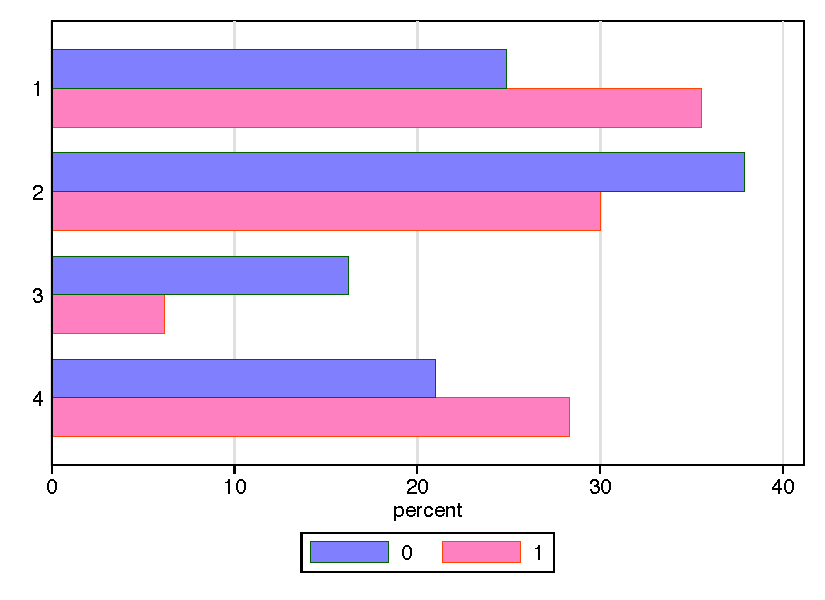
\includegraphics[scale = 0.7]{images/status.pdf}
\end{frame}

\begin{frame}{Distribution by education}
    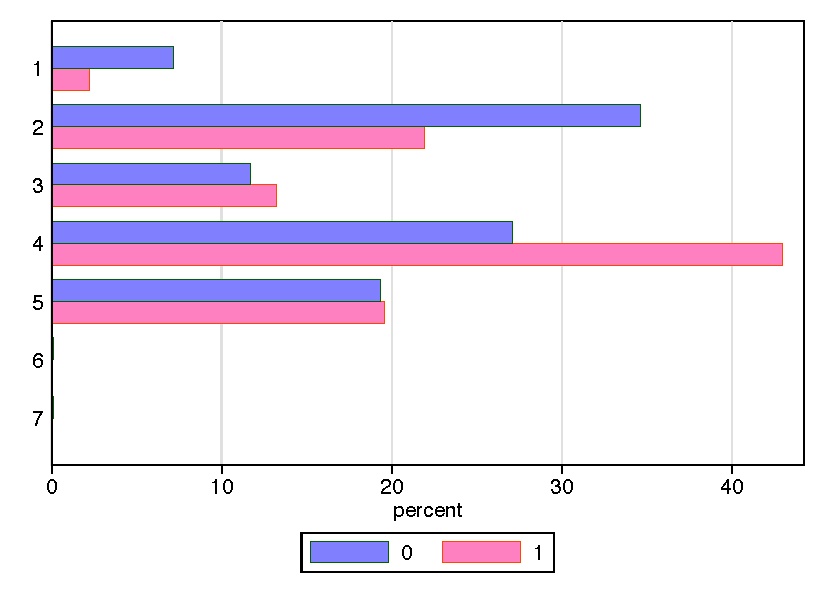
\includegraphics[scale = 0.7]{images/obrzw.pdf}
\end{frame}

\begin{frame}{Distribution by unemployment category}
    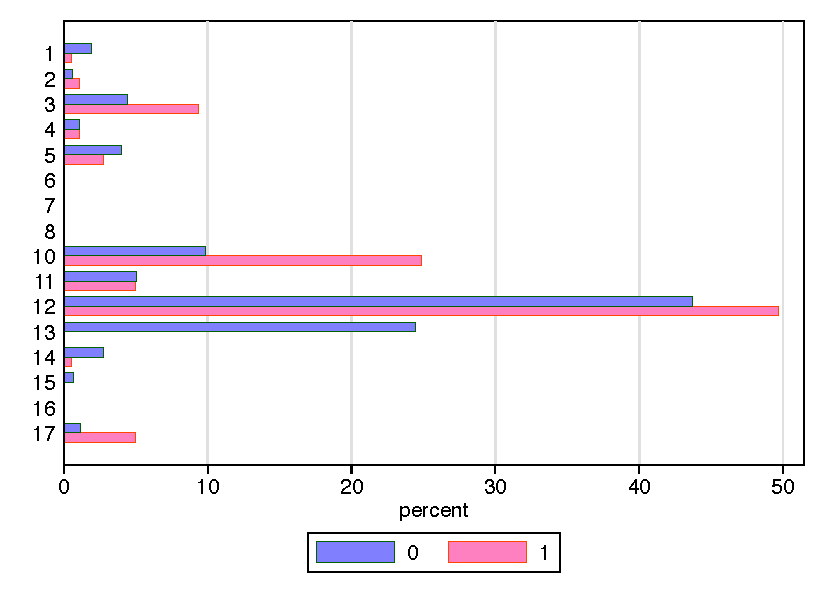
\includegraphics[scale = 0.7]{images/unem_cat.pdf}
\end{frame}


%---------------------------------------------------------------------------

\section{Analysis}

\begin{frame}{Before estimation}
    \centering
    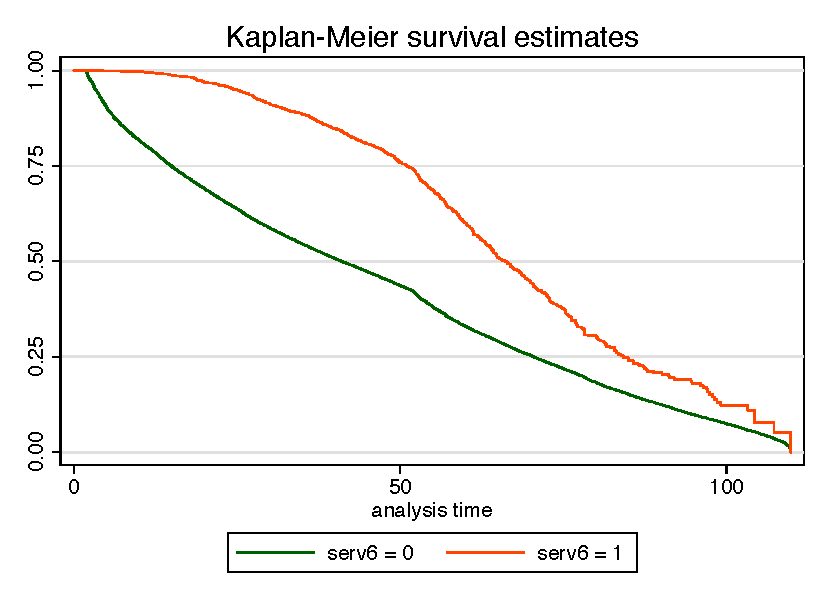
\includegraphics[scale=0.7]{images/surv_fun.pdf}
\end{frame}




%---------------------------------------------------------------------------

\begin{frame}{Adding controls}
\centering
{
\def\sym#1{\ifmmode^{#1}\else\(^{#1}\)\fi}
\begin{tabular}{l*{3}{c}}
\toprule
                &\multicolumn{1}{c}{Cox}&\multicolumn{1}{c}{Cox}&\multicolumn{1}{c}{Cox}\\
\cmidrule{2-4}
 & (1) & (2) & (3) \\
\midrule
=1 if Klub Ishushikh rabotu&    -0.87***&    -0.82***&    -0.87***\\
                &  (0.054)   &  (0.054)   &  (0.055)   \\
\addlinespace
number of dependants&    -0.26***&    -0.26***&    -0.24***\\
                & (0.0077)   & (0.0077)   & (0.0078)   \\

\midrule 
Age & Yes & Yes & Yes \\
Education & Yes & Yes & Yes \\
Unemployment status & No & Yes & Yes \\
District FE & No & No & Yes \\
\midrule
Observations    &    89137   &    89043   &    89043   \\
\bottomrule
\end{tabular}
}


\end{frame}



%---------------------------------------------------------------------------

\begin{frame}{Reduced sample}
\centering
\resizebox{0.9\linewidth}{!}{
\begin{tabular}{l*{3}{c}}
\toprule
                &\multicolumn{1}{c}{Weibull}&\multicolumn{1}{c}{Cox}&\multicolumn{1}{c}{Weibull}\\
                \cmidrule{2-4}
                \scriptsize{ & (1) & (2) & (3)} \\
\midrule

=1 if Klub Ishushikh rabotu&    -0.96&    -0.95&    -1.07\\
                &  (0.059)&  (0.059)&  (0.062)\\
\addlinespace
number of dependants&    -0.27&    -0.26&    -0.39\\
                & (0.0082)& (0.0082)&  (0.011)\\

\midrule
Age, education & Yes & Yes & Yes \\
Unemployment status & No & Yes & Yes \\
District FE & No & No & Yes \\
Unobserved heterogeneity & No & No & Yes \\
Weeks $< 70$ & Yes & Yes & No \\
\midrule
Observations    &    81311&    81311&    89043\\
\bottomrule
\end{tabular}

}
\end{frame}

%---------------------------------------------------------------------------

\begin{frame}{Adding controls (without ivdiwen)}
\centering
\resizebox{0.9\linewidth}{!}{
\begin{tabular}{l*{3}{c}}
\toprule
                &\multicolumn{1}{c}{Weibull}&\multicolumn{1}{c}{Cox}&\multicolumn{1}{c}{Weibull}\\
                \cmidrule{2-4}
                \scriptsize{ & (1) & (2) & (3)} \\
\midrule

=1 if Klub Ishushikh rabotu&    -0.88&    -0.89&    -0.94\\
                &  (0.039)&  (0.039)&  (0.039)\\
                
\midrule                
Age, education & Yes & Yes & Yes \\
Unemployment status & No & Yes & Yes \\
District FE & No & No & Yes \\
Unobserved heterogeneity & No & No & Yes \\
Weeks $< 70$ & Yes & Yes & No \\

\midrule
Observations    &   126873&   126873&   140486\\
\bottomrule
\end{tabular}

}

\end{frame}

%---------------------------------------------------------------------------

\begin{frame}{Survival function (Cox)}
\begin{figure}[ht]
        \begin{minipage}[b]{0.45\linewidth}
            \centering
            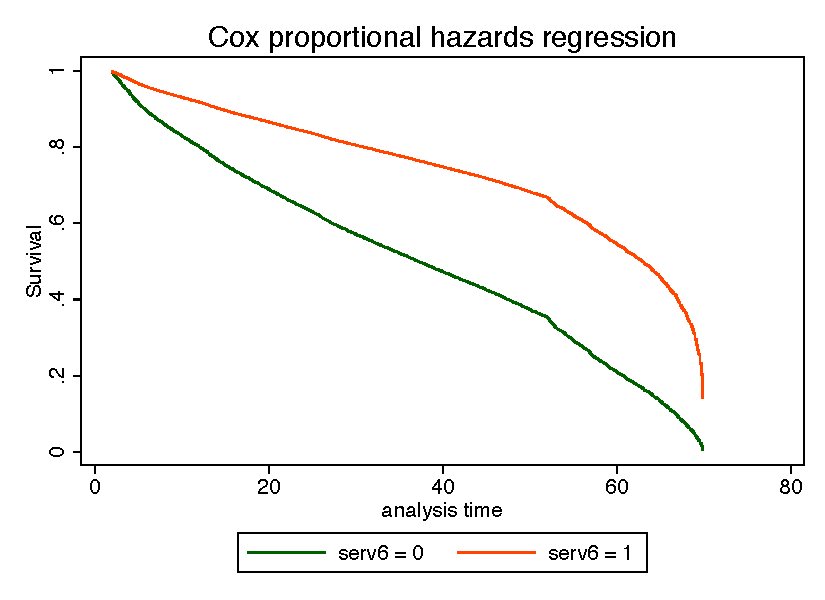
\includegraphics[width=\textwidth]{images/surv_cos.pdf}
            \caption{Reduced sample}
        \end{minipage}
        \hspace{0.5cm}
        \begin{minipage}[b]{0.45\linewidth}
            \centering
            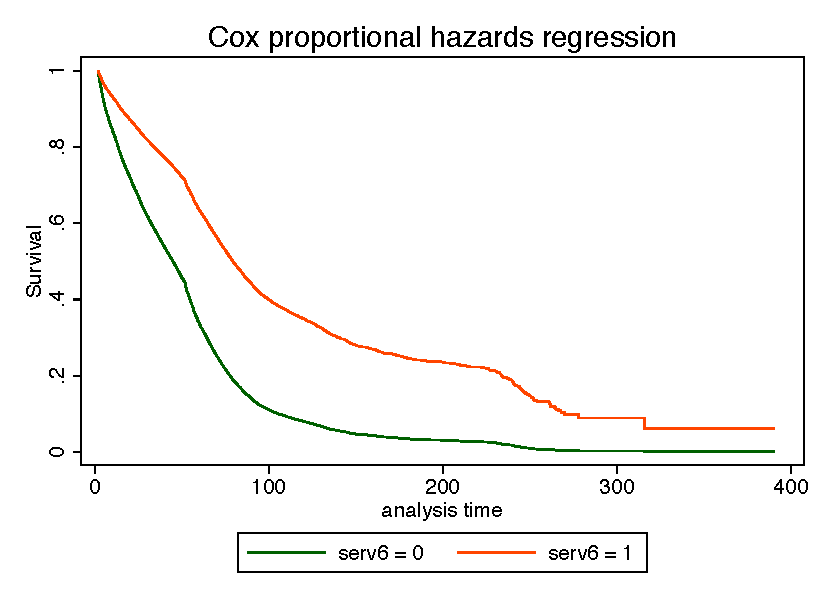
\includegraphics[width=\textwidth]{images/surv_cos_full.pdf}
            \caption{Full sample}
        \end{minipage}
    \caption{Survival function after Cox estimation (reduced sample, control for unemployment status, district fixed effects, and other controls).}
    \end{figure}

\end{frame}

%---------------------------------------------------------------------------

\begin{frame}{Attempt at finding a control group}
\centering
\resizebox{0.9\linewidth}{!}{
\begin{tabular}{l*{4}{c}}
\toprule
               & Redundant & Migrated & Redundant & Migrated \\ 
               \cmidrule{2-5} &\multicolumn{1}{c}{(1)}&\multicolumn{1}{c}{(2)}&\multicolumn{1}{c}{(3)}&\multicolumn{1}{c}{(4)}\\
\midrule
=1 if Klub Ishushikh rabotu&    -0.84&    -1.67&    -1.07&    -1.89\\
                &   (0.11)&   (0.43)&   (0.12)&   (0.47)\\
\addlinespace
number of dependants&   -0.071&    -0.14&   -0.070&    -0.17\\
                &  (0.015)&  (0.074)&  (0.017)&  (0.076)\\
\midrule
Age, education & Yes & Yes & Yes & Yes \\
Unemployment status & Yes & Yes & Yes & Yes \\
District FE & Yes & Yes & Yes & Yes \\
Weeks $< 70$ & No & No & Yes & Yes \\
\midrule
Observations    &    21280&      850&    17553&      777\\
\bottomrule
\end{tabular}

}

\end{frame}

%---------------------------------------------------------------------------

\begin{frame}{Full output for Weibull}

\centering

\adjustbox{
max totalheight=\textheight, max width=\textwidth, keepaspectratio}{
    {
\def\sym#1{\ifmmode^{#1}\else\(^{#1}\)\fi}
\begin{tabular}{l*{3}{c}}
\toprule
                &\multicolumn{1}{c}{1}&\multicolumn{1}{c}{2}&\multicolumn{1}{c}{3}\\
\midrule
main            &            &            &            \\
=1 if Klub Ishushikh rabotu&    -0.85***&    -0.82***&    -1.07***\\
                &  (0.054)   &  (0.054)   &  (0.062)   \\
\addlinespace
number of dependants&    -0.27***&    -0.26***&    -0.39***\\
                & (0.0077)   & (0.0077)   &  (0.011)   \\
\addlinespace
obrzw==     1.0000&     0.10***&     0.10***&     0.14***\\
                &  (0.020)   &  (0.020)   &  (0.026)   \\
\addlinespace
obrzw==     3.0000&     0.12***&     0.13***&    0.066***\\
                &  (0.017)   &  (0.017)   &  (0.021)   \\
\addlinespace
obrzw==     4.0000&    -0.20***&    -0.19***&    -0.32***\\
                &  (0.012)   &  (0.012)   &  (0.016)   \\
\addlinespace
obrzw==     5.0000&    -0.23***&    -0.22***&    -0.34***\\
                &  (0.013)   &  (0.013)   &  (0.018)   \\
\addlinespace
obrzw==     6.0000&     0.27*  &     0.31** &     0.16   \\
                &   (0.15)   &   (0.15)   &   (0.20)   \\
\addlinespace
obrzw==     7.0000&    0.029   &  0.00064   &   -0.067   \\
                &   (0.13)   &   (0.13)   &   (0.16)   \\
\addlinespace
agecat==     2.0000&    -0.21***&    -0.20***&    -0.20***\\
                &  (0.021)   &  (0.021)   &  (0.026)   \\
\addlinespace
agecat==     3.0000&    -0.20***&    -0.19***&    -0.15***\\
                &  (0.026)   &  (0.026)   &  (0.033)   \\
\addlinespace
agecat==     4.0000&    -0.11***&    -0.10***&   -0.052   \\
                &  (0.026)   &  (0.026)   &  (0.033)   \\
\addlinespace
agecat==     5.0000&    -0.32***&    -0.31***&    -0.32***\\
                &  (0.025)   &  (0.025)   &  (0.032)   \\
\addlinespace
agecat==     6.0000&    -0.70***&    -0.70***&    -0.82***\\
                &  (0.030)   &  (0.030)   &  (0.037)   \\
\addlinespace
agecat==     7.0000&    -0.94***&    -0.93***&    -0.98***\\
                &  (0.043)   &  (0.043)   &  (0.051)   \\
\addlinespace
agecat==     8.0000&  -0.0071   &    0.017   &     0.30***\\
                &  (0.060)   &  (0.060)   &  (0.074)   \\
\midrule
Observations    &    89043   &    89043   &    89043   \\
\bottomrule
\end{tabular}
}

    }

\end{frame}


%----------------------------------------------------------------------------



\end{document}
%---------------------------------------------------------------------------
